\section{Verbesserte Lösung
\label{perturbation:section:verbesserte_loesung}}
\rhead{Verbesserte Lösung}

Anstelle lediglich den Anfangswert $v_0$ anzupassen, erhält man bessere Resultate, indem auch $\vec{r} = (x_0, y_0)$ variabel gestaltet wird. 
Zudem kann man anstelle von $t$ nur die Differenz seit dem letzten Update der Bodenstation $\Delta t$ betrachten.

Wiederum ist das Ziel, dass der Flugkörper mit den einfachen Formeln \ref{eq:x_simple} und \ref{eq:y_simple} eine möglichst gute Approximation auf einfache Art und Weise berechnen kann, indem er die Anfangswerte $\vec{r}$ und $\vec{v}$ im Laufe der Zeit gemäss Weisungen der Bodenstation anpasst.

In einem ersten Schritt verlangen wir von der Bodenstation, welche $\vec{r}$, aber auch $\vec{v}$ mit Runge Kutta berechnen kann, ebendiese Werte um so eine Approximation mit den simplen Formeln \ref{eq:x_simple} und \ref{eq:y_simple} tätigen zu können. Es ergeben sich folgende Formeln:

\begin{equation}
    x(t + \Delta t) = x_0 + v_{0_x}\Delta t
\end{equation}
\begin{equation}
    y(t + \Delta t) = y_0 + v_{0_y}\Delta t - \frac{1}{2}g\Delta t^2
\end{equation}

Verlangt man von der Bodenstation jede Sekunde neue Werte für die oskulierenden Elemente $x_0, y_0, v_{0_x}$ und $v_{0_y}$ gibt dies eine Genauigkeit von 2 Stellen. In Abbildung \ref{error} ist der Fehler ersichtlich. Dieser ist als euklidische Distanz zur effektiven Position dargestellt.

\begin{figure}
    \centering
    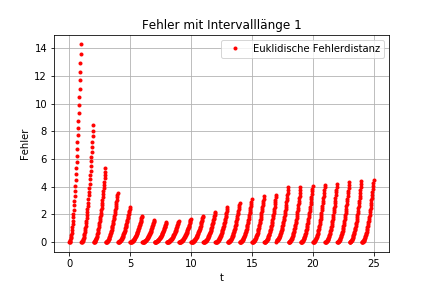
\includegraphics[scale = 0.7]{papers/perturbation/bilder/Ansatz2_Ordnung0_Errors.png}
    \caption{Fehler als euklidische Distanz}
	\label{error}
\end{figure}